\documentclass{winnower}
\lhead[]{}
\fancyhf{} % sets both header and footer to nothing
\renewcommand{\headrulewidth}{0pt}
\begin{document}

\title{%
  Generative Adversarial Network Tutorial \\
    \large Theories \& Models \& Applications \& Evaluations}

\author{Ahmed H. Al-Ghidani \\ Supervised by Prof. Aly Fahmy \\ Cairo University}

\maketitle

\date{}

\maketitle

\begin{abstract}
Generative Adversarial Network(GAN) is a newly invented technique and architecture that is considered to be a Neural-based model. GAN is basically dominating the Machine Learning and Deep Learning field nowadays and it is being used in many applications as a powerful Generative Model that can learn the dataset statistical distribution and generate other samples that have the same original distribution. 

On this survey, we try to illustrate and discuss this model, alongside its variations, and its applications on different fields. Basically, it is being used a lot in Computer Vision (CV) nowadays and they are investigating its capabilities in Natural Language Processing(NLP) and Generation(NLG). So, on this document, we will begin by defining the GAN model and shows the basic structure and loss function, followed by several other variations of the basic model and their applications with experiments on popular datasets (most of them are images datasets).
\end{abstract}


%-------------------------------------------------%
\section{Concepts and Terminologies}
%-------------------------------------------------%

Before going into the model theory, we need to illustrate and define some relevant terminologies and concepts that are considered to be the main backbone of GANs.\newline

\textbf{Discriminator Models:} Models that predict a hidden observation (called class) given some evidence (called features). In other words, we have some features and observations about an entity, and we want to predict its class, category or label. You can imagine the model as a function that has features as input and produces an output. The criteria that is used to produce the output depends on the model architecture and nature. So, the discriminative model could be described in mathematical formula by \(f(x_1, x_2, .., x_n) = y\), where \textbf{n} is the number of features, and the target of the function is to get the conditional probability \(P(Y|x_1, x_2, .., x_n)\). \textbf{Support Vector Machines (SVMs)} and \textbf{Deep Neural Networks (DNNs)} are examples of discriminative models that are used for classification.\newline

\textbf{Generative Models:} Given some features, the models target is to learn how these features are produced, it tries to learn the distribution of the features. Assume that we have features \(x_1, x_2, x_3, …, x_n\) where \textbf{n} is the number of features, the model targets to learn the joint probability distribution of the features with the classes. We can formulate this in mathematics by the joint probability \(P(x1, x2, x3, …, xn, y\). After learning this distribution, we can estimate the conditional probability of the discriminative models to get the probability of the class given these features with their distribution. \textbf{Restricted Boltzmann Machines (RBMs)} and \textbf{Hidden Markov Models (HMMs)} are examples of generative models. Note that, \textbf{Vanilla Autoencoders (AEs)} aren’t considered to be a generative model, all what they do is just reconstruction of the features, on the other hand, \textbf{Variational Autoencoders (VAEs)} belongs to generative models family. \newline

\textbf{Nash Equilibrium:} A conceptual term that is used in \textbf{Game Theory} to describe a game situation in which the game players are satisfied by the decision he/she makes after revealing the other players strategies, and each player has no intention to change the strategy after knowing the other strategies as they didn’t effect on the strategy he/she used to win the game.

For example, assume we have a game in which each player has 2 choices to choose between them, and the 2 choices are known that are right and have the same effect regarding to the game points or rewards. The first player strategy maybe to choose the first choice, while the other player’s choice is the second one. After revealing that, each player is satisfied by the strategy he/she took because the other’s choice hasn’t effect badly to him/her. \newline

\textbf{Minimax:} An algorithm that belongs to Game Theory and Statistics. The algorithm is used in games in which the game participants are 2 players, and each player tries to win the game by minimizing the worst case that is provided by the other player move, in other words, the player Minimize the Maximum move of the other player.

You can imagine the game of Chess, in which each player tries to win by making the best available move while the other player tries to minimize this move which is considered to be the best move by his side. Minimax is commonly used when making an AI-bot agent in Chess, Tic-tac-toi and Connect-4 games, you can generalize in the decision-making rule-based games.


%-------------------------------------------------%
\section{Introduction to Generative Adversarial Network}
%-------------------------------------------------%
\begin{center}
  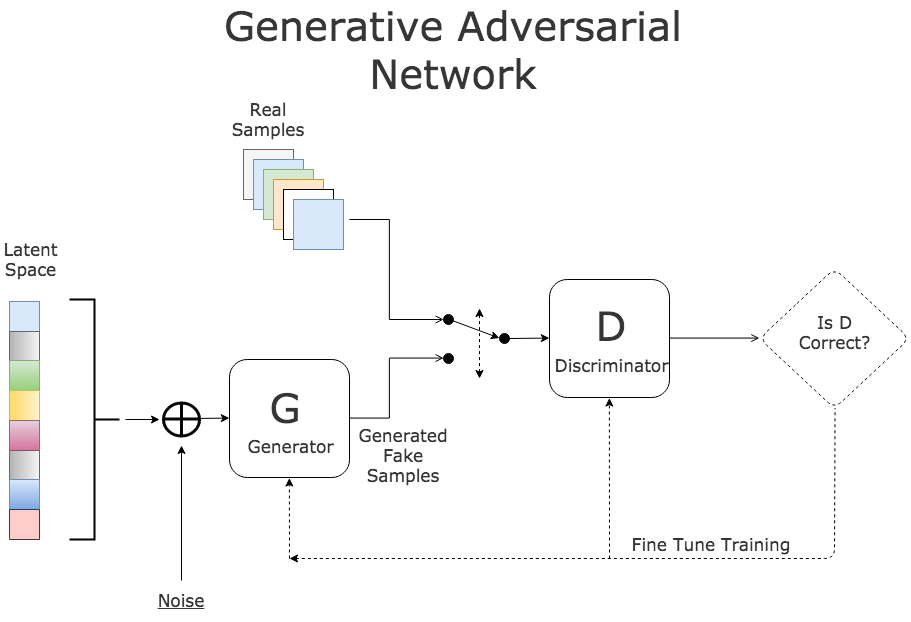
\includegraphics[width=13cm, height=8cm]{gan.png}
\end{center}

\textbf{GAN} consists of 2 models, a discriminative model (D) and a generative model (G). These models are participants on the training phase which looks like a game between them, and each model tries to better than the other. The target of the generative model is to generate samples that are considered to be fake and are supposed to have the same distribution of the original data samples, on the other hand, the discriminative’s target is to enhance itself to be able to recognize the real samples among the fake samples generated by the generative model. It looks like a game, in which each player (model) tries to be better than the other, the generative model tries to generate samples that deceives and tricks the discriminative model, while the discriminative model tries to get better in recognizing the real data and avoid the fake samples. It is as mentioned before, it is the same idea of the Minimax algorithm, in which each player targets to fail the other and minimize the supposed loss.\newline

This game continues till we get a state, in which each model becomes an expert on what it is doing, the generative model increases its ability to get the actual data distribution and produces data like it, and the discriminative becomes expert in identifying the real samples, which increases the system’s classification task. In such case, we know that it reached that in which each model satisfied by its output (strategy), which is called \textbf{Nash Equilibrium} in Game Theory. During the training phase, the loss function, that calculates the error, is used to update the 2 models parameters (learning the weights), also, the model can’t change the other’s parameters, the parameters are locally updated in each model using the global error.

%-------------------------------------------------%
\subsection{Maximum Likelihood Generative Models}
%-------------------------------------------------%

Assume that we have a dataset that contains m training samples, these samples follow an unknown probability distribution, it could be \textbf{Gaussian}, \textbf{Bernoulli} or any other probability distribution, actually, we don’t care about knowing such distribution. Our focus is to be able to generate similar data that has the same distribution of the training dataset. We can formulate the problem as a Maximum Likelihood Estimation problem.\newline

The idea of Maximum Likelihood is to make a model that has some parameters which make it be able to generate the same probability distribution \[Pmodel(X;\theta)\]. As we we have \textbf{m} samples in the training data, we can generalize the Maximum Likelihood all over the data \[\prod_{i = 1}^m Pmodel(X_i;\theta)\]

Now, the target is to find \(\theta\) that Maximize the likelihood, so, our mathematical representation of this problem would be \[\theta:=argmax_\theta \prod_{i = 1}^m Pmodel(X_i;\theta)\]

To avoid any numerical problems, it is always better to transform to the \textit{log} space, as you know, \[\textit{log(x * y)} = \textit{log(x)} + \textit{log(y)}\]. 
We turn the above equation to sum instead of product. So, our final Empirical Distribution equation to obtain the Maximum Likelihood of the training data will be \[\theta:=argmax_\theta \sum_{i = 1}^m log(Pmodel(X_i;\theta))\]

We call the above model as an \textbf{Empirical Distribution}, as we don’t pretty certain about the distribution we get after getting the parameter \(\theta\). The question is, how to know whether the obtained distribution is really the actual distribution of the training data?\newline

\textbf{Kullback–Leibler Divergence (KL-divergence)} is a distance metric that could be used to answer the above question, and it can be used in both the discrete and continuous probability distributions. Given 2 probability distributions, \(P\) and \(Q\), the \textbf{KL-divergence} is measured by \[KL(P\|Q) = \sum_{i = 1}^{n} P(i) * log(\frac{P(i)}{Q(i)})\].

The target is to minimize the \textbf{KL-divergence}, the less difference between the distributions of \(P\) and \(Q\) means that they are close to each other. So, recall our Maximum Likelihood, after getting the empirical distribution, we measure the \textbf{KL-divergence} between the empirical distribution and the actual distribution, in other words, minimizing the \textbf{KL-divergence} means maximizing the Likelihood of the training dataset.

%-------------------------------------------------%
\subsection{Explicit vs. Implicit Maximum Likelihood Models}
%-------------------------------------------------%
After knowing the general idea of Maximum Likelihood models and their target, we need to be more specified when we consider talking about Maximum Likelihood generative models. Actually, there are 2 different types of Maximum Likelihood models, Explicit and Implicit models.\newline

\textbf{Explicit Models:} Models that fully depend on the training data, and try to learn the parameters of \(P(X;\theta)\), which are the mean and variance, using the regular gradient or any other optimization technique. To be able to make the training efficient, we need to design a model that makes use of the training samples, also, the collected training samples should be generalized enough to cover all variables of the probability distribution and this may be hard in some real-life data, finally, the explicit models require some complex computational power to learn the parameters.\newline

\textbf{Implicit Models:} In these models, we don’t actually use the data to learn the true distribution parameters, we assume that the distribution parameters are hidden and we try to predict it using some observed variables from the data. These observed variables have no rules to be determined, they are extracted by the researcher or by an expert who may have a pre-knowledge about the data. You can think of it as an inference stochastic process that could be done using Markov Chains, you use some observable data to be able to get the hidden variables (called Latent variables), refer to this post to know more about Markov Chains. We use these latent variables (which makes a latent space) to generate a similar data based on the given training samples. Regularly, implicit models could be used for dimension reduction of the data without any prior knowledge about the data distribution.\newline

GAN uses the latent space to be able to generate data that is considered to be in similar distribution of the real samples. So, it is an implicit model, but it doesn’t use any observable data like \textbf{Markov Chains} do, it deals directly with the training sample, in other words, it treats the samples of the training data as the latent variables, and change their distribution by adding some noise to the sample features. That’s why it is considered to be an implicit model, it doesn’t use the data distribution, and it doesn’t depend on any observable data, like we do with Markov Chains.\newline

To clarify more, you can imagine the situation by learning without any prior knowledge about something, you just do mistakes and you let others correct them to you. Continuing this process will lead you to learn how to do that thing, although you may still don’t know what are you doing?!\newline

Actually, there are many different types of Maximum Likelihood models in general, the following figure is a taxonomy of different types of models.\newline
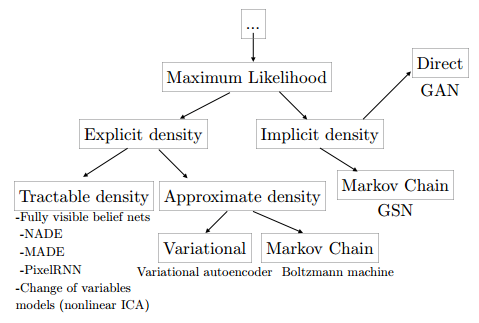
\includegraphics[width=17cm, height=10cm]{taxo.png}

%-------------------------------------------------%
\section{Adversarial Process}
%-------------------------------------------------%	
Typically, in basic GAN architectures (there are other variations that we will discuss later), you are given a dataset that contains some training examples, these examples follow some known or unknown probability distributions, these distributions could be unimodal (single distribution) or multi-modal (two or more complex distributions). The following figure shows 2 probability distributions to clarify more.

\begin{center}
  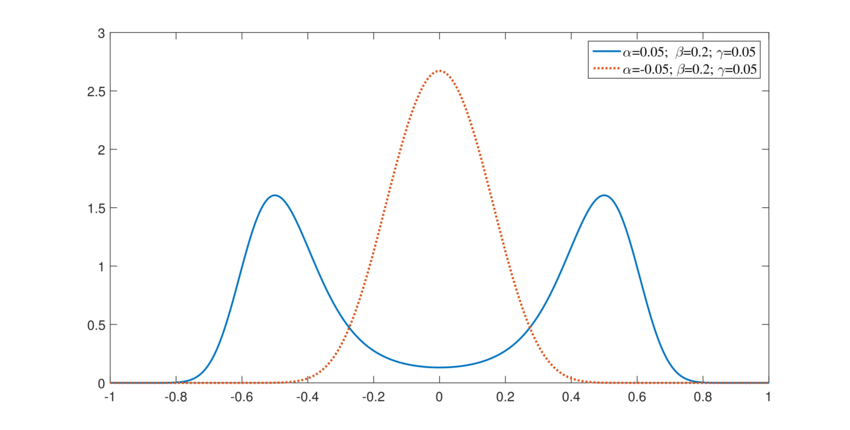
\includegraphics[width=15cm, height=10cm]{dists.png}
\end{center}

The model complexity depends on the number of similar samples in the data, which is knows as the number of classes. In Supervised Learning, each class samples have a specific distribution (that's why they are labeled by the same class) that differs it from the other classes samples distribution. GAN tries to model these distributions by transforming a latent space from another distribution to the data distribution. In practice, it is maybe hard to model 1 latent space to multi-modal space that make GAN falls as a prey to the \textit{Mode Collapse} problem. We will dive into it later.\newline

Concretely, lets assume that we have a dataset of images. We want to build a GAN to be able generate fake images by learning these images data distribution. The following figure shows how the model processes.

\begin{center}
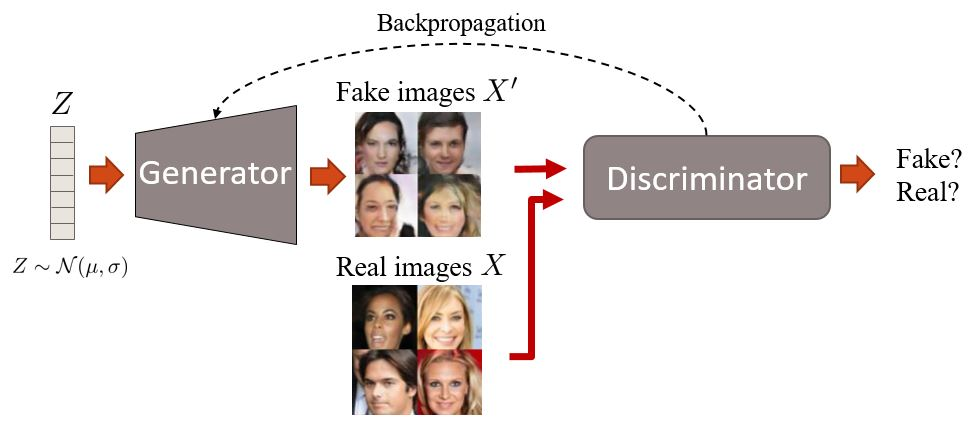
\includegraphics[width=15cm, height=8cm]{train.jpg}
\end{center}

Lets use some mathematical notations to be able to formalize our problem. As we have mentioned above, we 2 types of models in GAN, the discriminator D and the generator G. The discriminator tries to distinguish between the real images D(x) and the fake generated images D(G(z)). The generator takes a latent space z and generates fakes images to fool the discriminator G(z). As it is a dual problem and we want to make the model converges, our function (called Jensen-Shannon divergence) that we want to optimize is \[min_G \\ max_D \\ E_{x\sim p(x)} [log D(x)] + E_{z\sim p(z)} [log(1 - D(G(z))] = \] \[min_G \\ max_D \\ E_{x\sim p(x)} [log D(x)] + E_{x\sim p_g(x)} [log(1 - D(x)]\]\newline

Let's take a closer look to the above equation. It consists of 2 parts \[E_{x\sim p(x)} [log D(x)]\] and \[E_{z\sim p(z)} [log(1 - D(G(z))]\]\newline

We maximize the first part as we want \(D(x)\) to be closer 1 which means that it recognizes the real image \(x\). The second part we minimize \(G(z)\) which means that it is getting close to \(0\). The above equation optimizes the discriminator at its point of view as a simple \textbf{Binary Cross Entropy (BCE)} function.

%-------------------------------------------------%
\subsection{Alternative Loss Function for Generator}
%-------------------------------------------------%
The above equation is formulated respected to the Discriminator point of view. Practically, they found that there may be a problem when updating the gradient for the Generator. When the Discriminator reaches its best state, it simply separate between the generated data and the real data, so, the quantity \(E_{z\sim p(z)} [log(1 - D(G(z))]\) vanishes through the training phase while the Generator tries to minimize it. Instead, we can just maximize \(E_{z\sim p(z)} [log(D(G(z))]\), this practically boosting the early gradients at the training phase. However, the researchers have no enough theoretical motivation to use it as it terminates the relation with Jensen-Shannon divergence, also it exploits the meaningful of the minimax game (as there is nothing to be minimized now!)\newline

Another alternative to the loss function formulation is to add the original loss function with the new rule above, so that it becomes \[\frac{E_{z\sim p(z)} [log(D(G(z))]}{E_{z\sim p(z)} [log(1 - D(G(z))]}\]

Note that, the above equation won't suffer from any kind of vanishing gradient as the division output will be unnormalized!

%-------------------------------------------------%
\subsection{Relation with Kullback-Leibler Divergence}
%-------------------------------------------------%

\textbf{Kullback-Leibler Divergence:} Measures how one probability distribution \(P\) diverges from a second expected probability distribution \(Q\). In this case, we will assume that \(Q\) is from the generative model. The KL-divergence equation for minimization will be \[KL(Q\|P) = E_{x \sim Q} log \frac{Q(x)}{P(x)}\]
As \(Q(x)\) is from the Generator and \(D(x)\) is the optimal distribution the we target, our equation could be \[E_{x \sim Q} log \frac{1 - D(x)}{D(x)}\] Which corresponds to the maximization equation above.

%-------------------------------------------------%
\section{Problems In Basic GANs}
%-------------------------------------------------%
As we have mentioned, training GANs is considered to be a hard task. There are reasons occur because of the training data nature and some others because of the method of training the model. Several modifications and variations have been developed to overcome some of the basic GAN common problems while in the training phase. We are going to illustrate some of them and their suggested solutions if they are available

%-------------------------------------------------%
\subsection{Mode Collapse}
%-------------------------------------------------%
In complex datasets, the data could be multi-modal distributed. As we know, the generator tries to transform from the latent space to the dataset distribution, but in the case of multi-modal, the generator could be biased towards one of the distribution instead of modeling the whole distribution. The following figure shows an example of bimodal data distribution of 2 classes.

\begin{center}
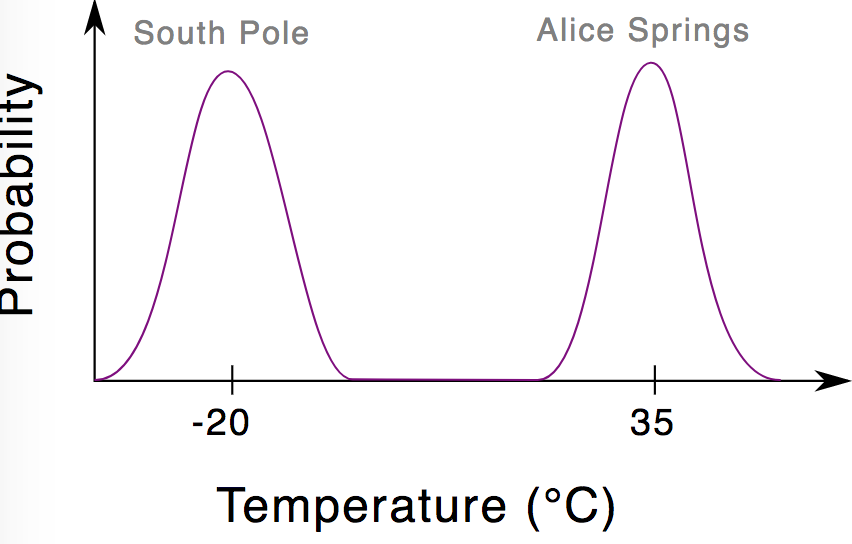
\includegraphics[width=14cm, height=10cm]{bimodal.png}
\end{center}

In such scenario, the generator can only learn to produce data from one of the distribution relying on that the discriminator only checks of the data generated is similar to the real data, it doesn't care about the generated classes. \newline

There are 3 known methods that we could be able to observe in our research (regardless the conditional variants of GAN). \newline

The first one is building \textbf{n} GANs model, where \textbf{n} is the number of data classes. By this, we avoid the problem from the beginning as each GAN will learn different distributions. As a trade off, this is considered to be a highly cost solution because we would need to create multiple GAN models to serve the classes. Another problem is that we need an annotated data to know the number of classes. \newline

The second ons is to train the model by batches and the number of classes of each batch is uniformly distributed over the batch. But also we need annotated data for this solution.


%-------------------------------------------------%
\subsection{Vanishing Gradient}
%-------------------------------------------------%

What if the Discriminator model is too powerful and always beats the Generator? Simply, the parameters update for the Generator won't be updated enough during the training data. So, when building the model, we need to make sure that there is an equilibrium between the 2 models and their complex structures

%-------------------------------------------------%
\subsection{High Dimensional Data}
%-------------------------------------------------%
The Generator maps between a known latent space distribution to the real data distribution. By intuition, it could be difficult to map low dimensional data with other data that is in a very high dimensions.


%-------------------------------------------------%
\section{Naive GAN Applications}
%-------------------------------------------------%
GAN is dominating the field of images. There are many attempts to generate images. However, there is no many application on the naive GAN, they prefer to use much more complex models, such as \textbf{Deep Convolutional GAN (DCGAN)} and \textbf{Adversarial Autoencoders}. The following examples are experiments from the original paper of GAN.

\begin{center}
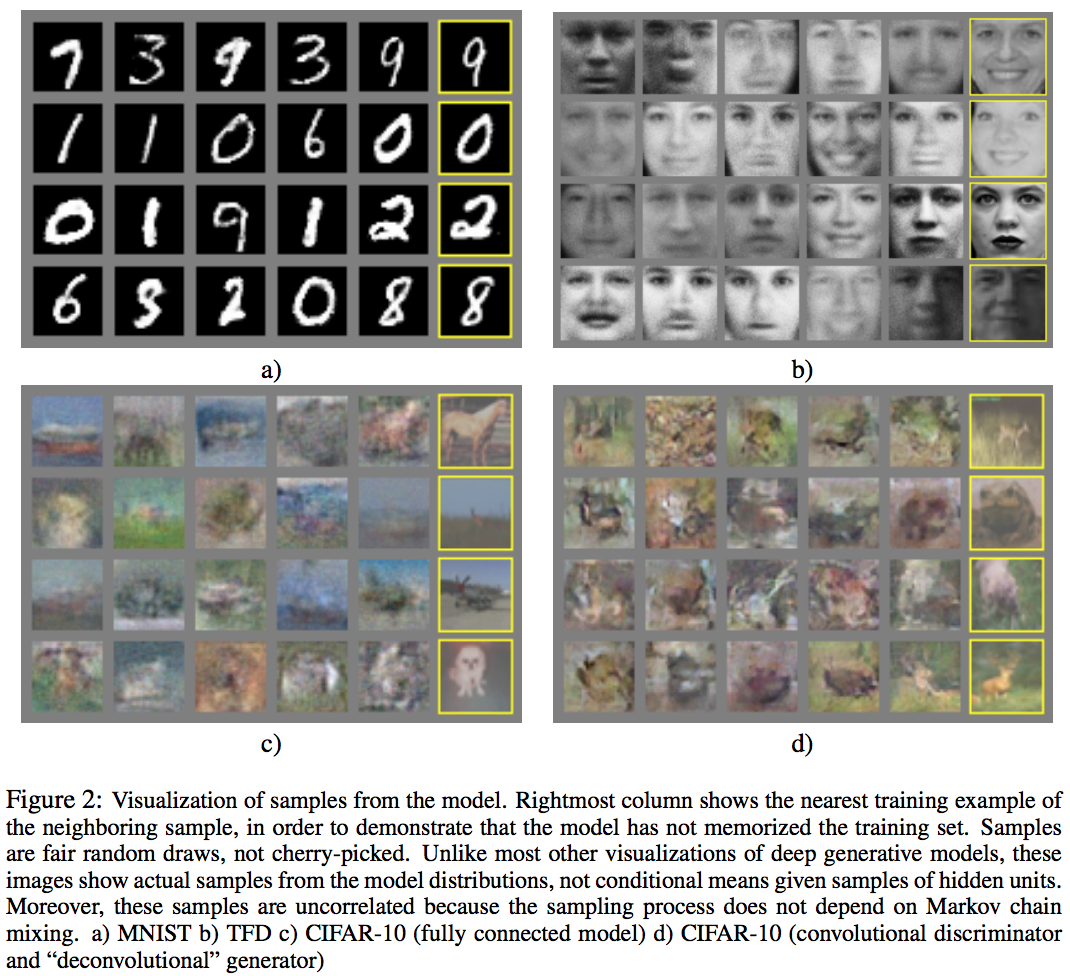
\includegraphics[width=12cm, height=12cm]{all.png}
\end{center}

%-------------------------------------------------%
\section{Conditional GAN (CGAN)}
%-------------------------------------------------%
This was a follow model after the original paper. The main difference between the naive GAN and the CGAN is that the generator takes a conditional features that help on generating the target entities. It is considered a prior knowledge that is given to the generator to help it on the generation process. The following figure shows an example CGAN that is conditioned under features \(y\)
\begin{center}
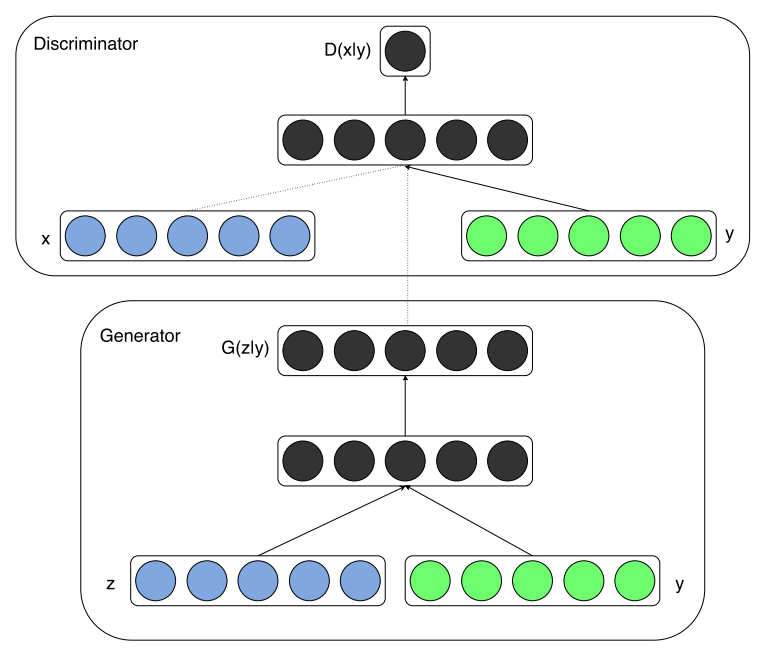
\includegraphics{cgan.png}
\end{center}

Thus, the cost function will updated like the following
\[min_G \\ max_D \\ E_{x\sim p(x)} [log D(x|y)] + E_{z\sim p(z)} [log(1 - D(G(z|y))]\]

The following figure shows the CGAN results on MIR Flickr 25,000 dataset

\begin{center}
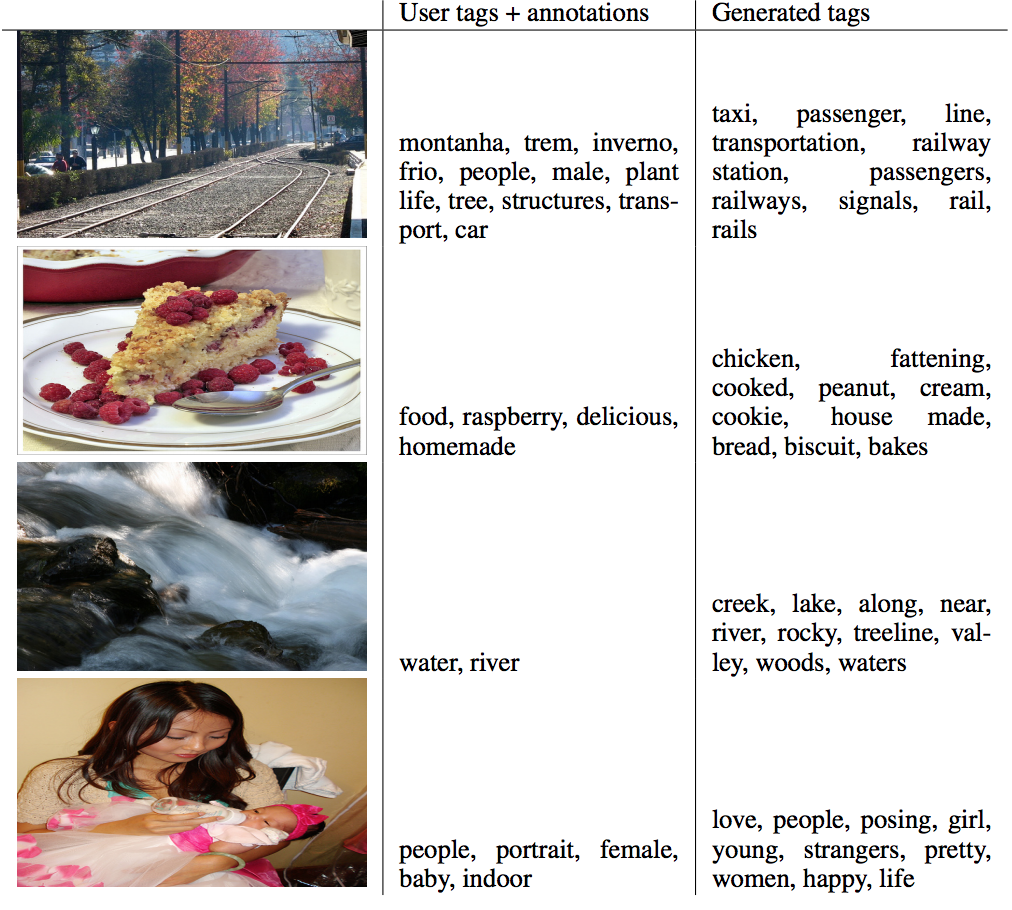
\includegraphics{flicker.png}
\end{center}

%-------------------------------------------------%
\section{Deep Convolutional GAN (DCGAN)}
%-------------------------------------------------%
Highly used in images. Using the power of \textbf{Convolutional Neural Network (CNN)}, DCGAN proved itself as a great GAN model that overcome some of the naive GAN problems. Both the Generator and Discriminator are CNN-based models. There is no major change in the loss function of the model. The following figure shows the Generator architecture. 

\begin{center}
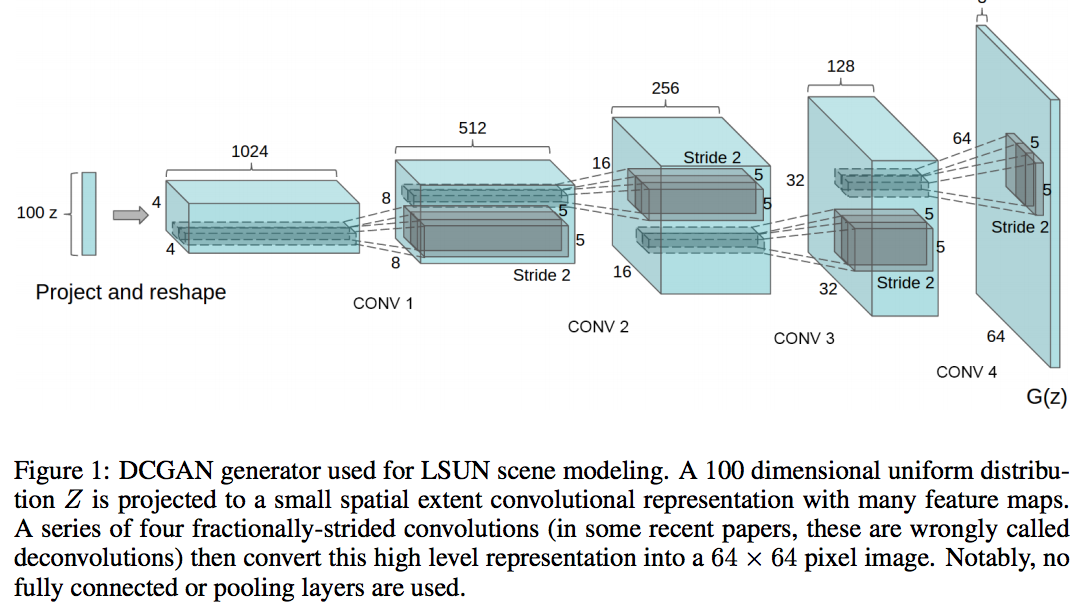
\includegraphics[width=16cm, height=9cm]{dcgan.png}
\end{center}

The following is an example of generated bedrooms images trained on LSUN dataset.

\begin{center}
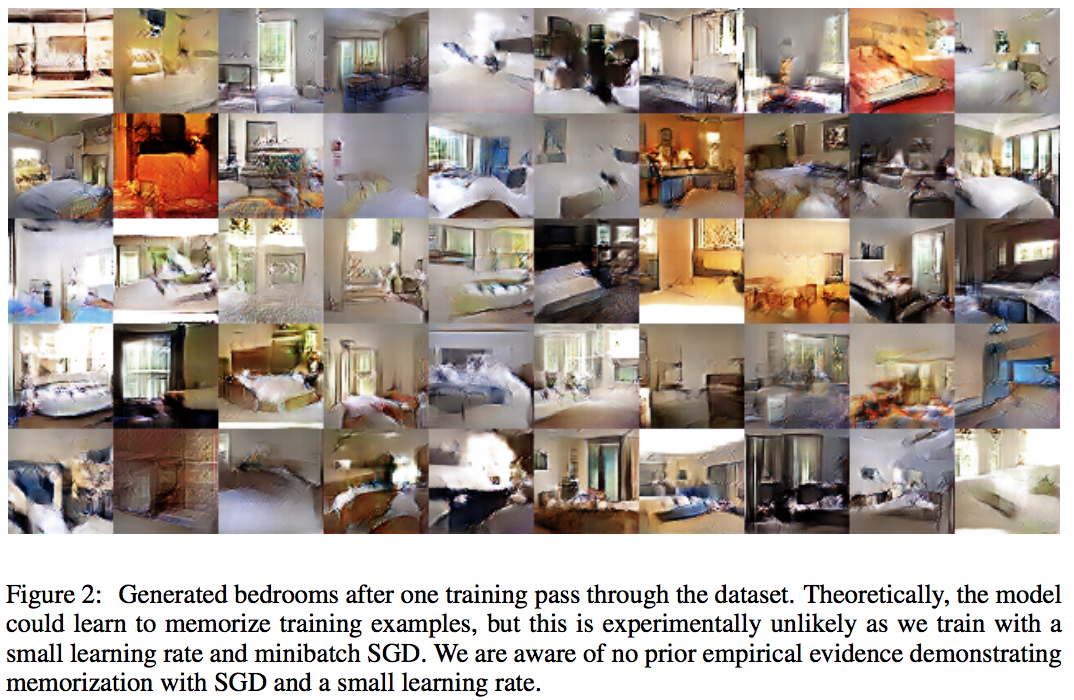
\includegraphics{bedrooms.png}
\end{center}

\bibliographystyle{abbrvnat}
\bibliography{winnower_template}
[1] Ian J. Goodfellow et al. "Generative Adversarial Networks". GAN \newline
[2] Mehdi Mirza and Simon Osindero. "Conditional Generative Adversarial Nets". CGAN \newline
[3] Alireza Makhzani et al. "Unsupervised Representation Learning with Deep Convolutional Generative Adversarial Networks". DCGAN \newline
[4] An Alternative Update Rule for Generative Adversarial Networks. http://www.inference.vc/an-alternative-update-rule-for-generative-adversarial-networks/ \newline
[5] Ian J. Goodfellow. NIPS 2016 Tutorial: Generative Adversarial Networks \newline
[6] from-GAN-to-WGAN. https://lilianweng.github.io/lil-log/2017/08/20/from-GAN-to-WGAN.html \newline
[7] Shibani Santurkar, Ludwig Schmidt, Aleksander M ˛adry. A CLASSIFICATION–BASED PERSPECTIVE ON GAN DISTRIBUTIONS \newline
[8] Martin Arjovsky Leon Bottou. TOWARDS PRINCIPLED METHODS FOR TRAINING GENERATIVE ADVERSARIAL NETWORKS \newline
[9] Martin Arjovsky, Soumith Chintala, Léon Bottou. Wasserstein GAN \newline
[10] Mode collapse in GANs. http://aiden.nibali.org/blog/2017-01-18-mode-collapse-gans/ \newline
[11] Fantastic GANs and where to find them http://guimperarnau.com/blog/2017/03/Fantastic-GANs-and-where-to-find-them \newline
[12] https://github.com/dongb5/GAN-Timeline \newline
[13] Wasserstein GAN https://vincentherrmann.github.io/blog/wasserstein/ \newline
[14] https://github.com/AhmedHani/really-awesome-gan \newline
[15] https://ahmedhanibrahim.wordpress.com/2017/01/17/generative-adversarial-networks-when-deep-learning-meets-game-theory/ \newline
[16] https://github.com/znxlwm/tensorflow-MNIST-GAN-DCGAN \newline
[17] GANs Foundation https://www.cs.toronto.edu/~duvenaud/courses/csc2541/slides/gan-foundations.pdf \newline
[18] JENSEN-SHANNON DIVERGENCE https://datawarrior.wordpress.com/tag/jensen-shannon-divergence/

\end{document}